%%%% acra.tex

\typeout{ACRA Instructions for Authors}

% This is the instructions for authors for ACRA.
\documentclass{article}
\usepackage{acra}
\usepackage{lmodern}% http://ctan.org/pkg/lm
\usepackage{amsmath}
\usepackage{graphicx}
\usepackage{color}
\usepackage{hyperref}
\usepackage{amssymb}
\usepackage{url}
\usepackage{pdfpages}
\usepackage{fancyhdr}
\usepackage{subfig}
\usepackage{listings} 
\usepackage{selinput}    
\usepackage{tikz}
\newcommand{\quotes}[1]{``#1''}

% The file acra.sty is the style file for ACRA. 
% The file named.sty contains macros for named citations as produced 
% by named.bst.

% The preparation of these files was supported by Schlumberger Palo Alto
% Research, AT\&T Bell Laboratories, and Morgan Kaufmann Publishers.
% Shirley Jowell, of Morgan Kaufmann Publishers, and Peter F.
% Patel-Schneider, of AT\&T Bell Laboratories collaborated on their
% preparation. 

% These instructions can be modified and used in other conferences as long
% as credit to the authors and supporting agencies is retained, this notice
% is not changed, and further modification or reuse is not restricted.
% Neither Shirley Jowell nor Peter F. Patel-Schneider can be listed as
% contacts for providing assistance without their prior permission.

% To use for other conferences, change references to files and the
% conference appropriate and use other authors, contacts, publishers, and
% organizations.
% Also change the deadline and address for returning papers and the length and
% page charge instructions.
% Put where the files are available in the appropriate places.

\title{Markov Chain Monte Carlo}
\author{Diego Garrido}

\begin{document}

\maketitle

Markov Chain Monte Carlo (MCMC) is one of the most used methods to approximate a complicated distribution. In this paper we use two MCMC algorithm, the Metropolis-Hastings algorithm and the Gibbs Sampling algorithm.

\href{https://nbviewer.jupyter.org/github/dgarridoa/MCMC_Py/blob/main/MCMC.ipynb}{\color{blue}{Jupyter Notebook}}

\section{Metropolis Hastings}

In this section we use the Metropolis-Hastings (MH) algorithm to approximate empirically the distribution $p(x) \propto 2e^{-(x-2)^{2}}+e^{-|x|}+e^{-(x+2)^{2}}e^{-|x+2|}=\tilde{p}(x)$. Firstly, we chose a proposal distribution with the same support as $p(x)$, as a Gaussian proposal, i.e., $q(x^{'}|x_{i})=\mathcal{N}(x_{i}, \sigma^{2})$. Since the proposal is symmetric, the acceptance probability is given by $\alpha=\min\big(1, \frac{\tilde{p}(x')}{\tilde{p}(x_{i})}\big)$. Secondly, we draws 5000 samples from $p(x)$ using MH with $\sigma\in\{0.01, 0.1, 1, 100\}$. This is ilustrated in Figure 1. Different choices of the proposal standard deviation $\sigma$ lead to very different results. If the proposal is too narrow, only one mode of $p(x)$ might be visited. On the other hand, if it is too wide, the rejection rate can be very high, resulting in high correlations. In sum, the success or failure of the algorithm not only depends on the choice of the proposal distribution, it also depends on its parameters, in this case the adecuate $\sigma$ might be in $\{0.1, 1\}$. 

\begin{figure}[!h]
    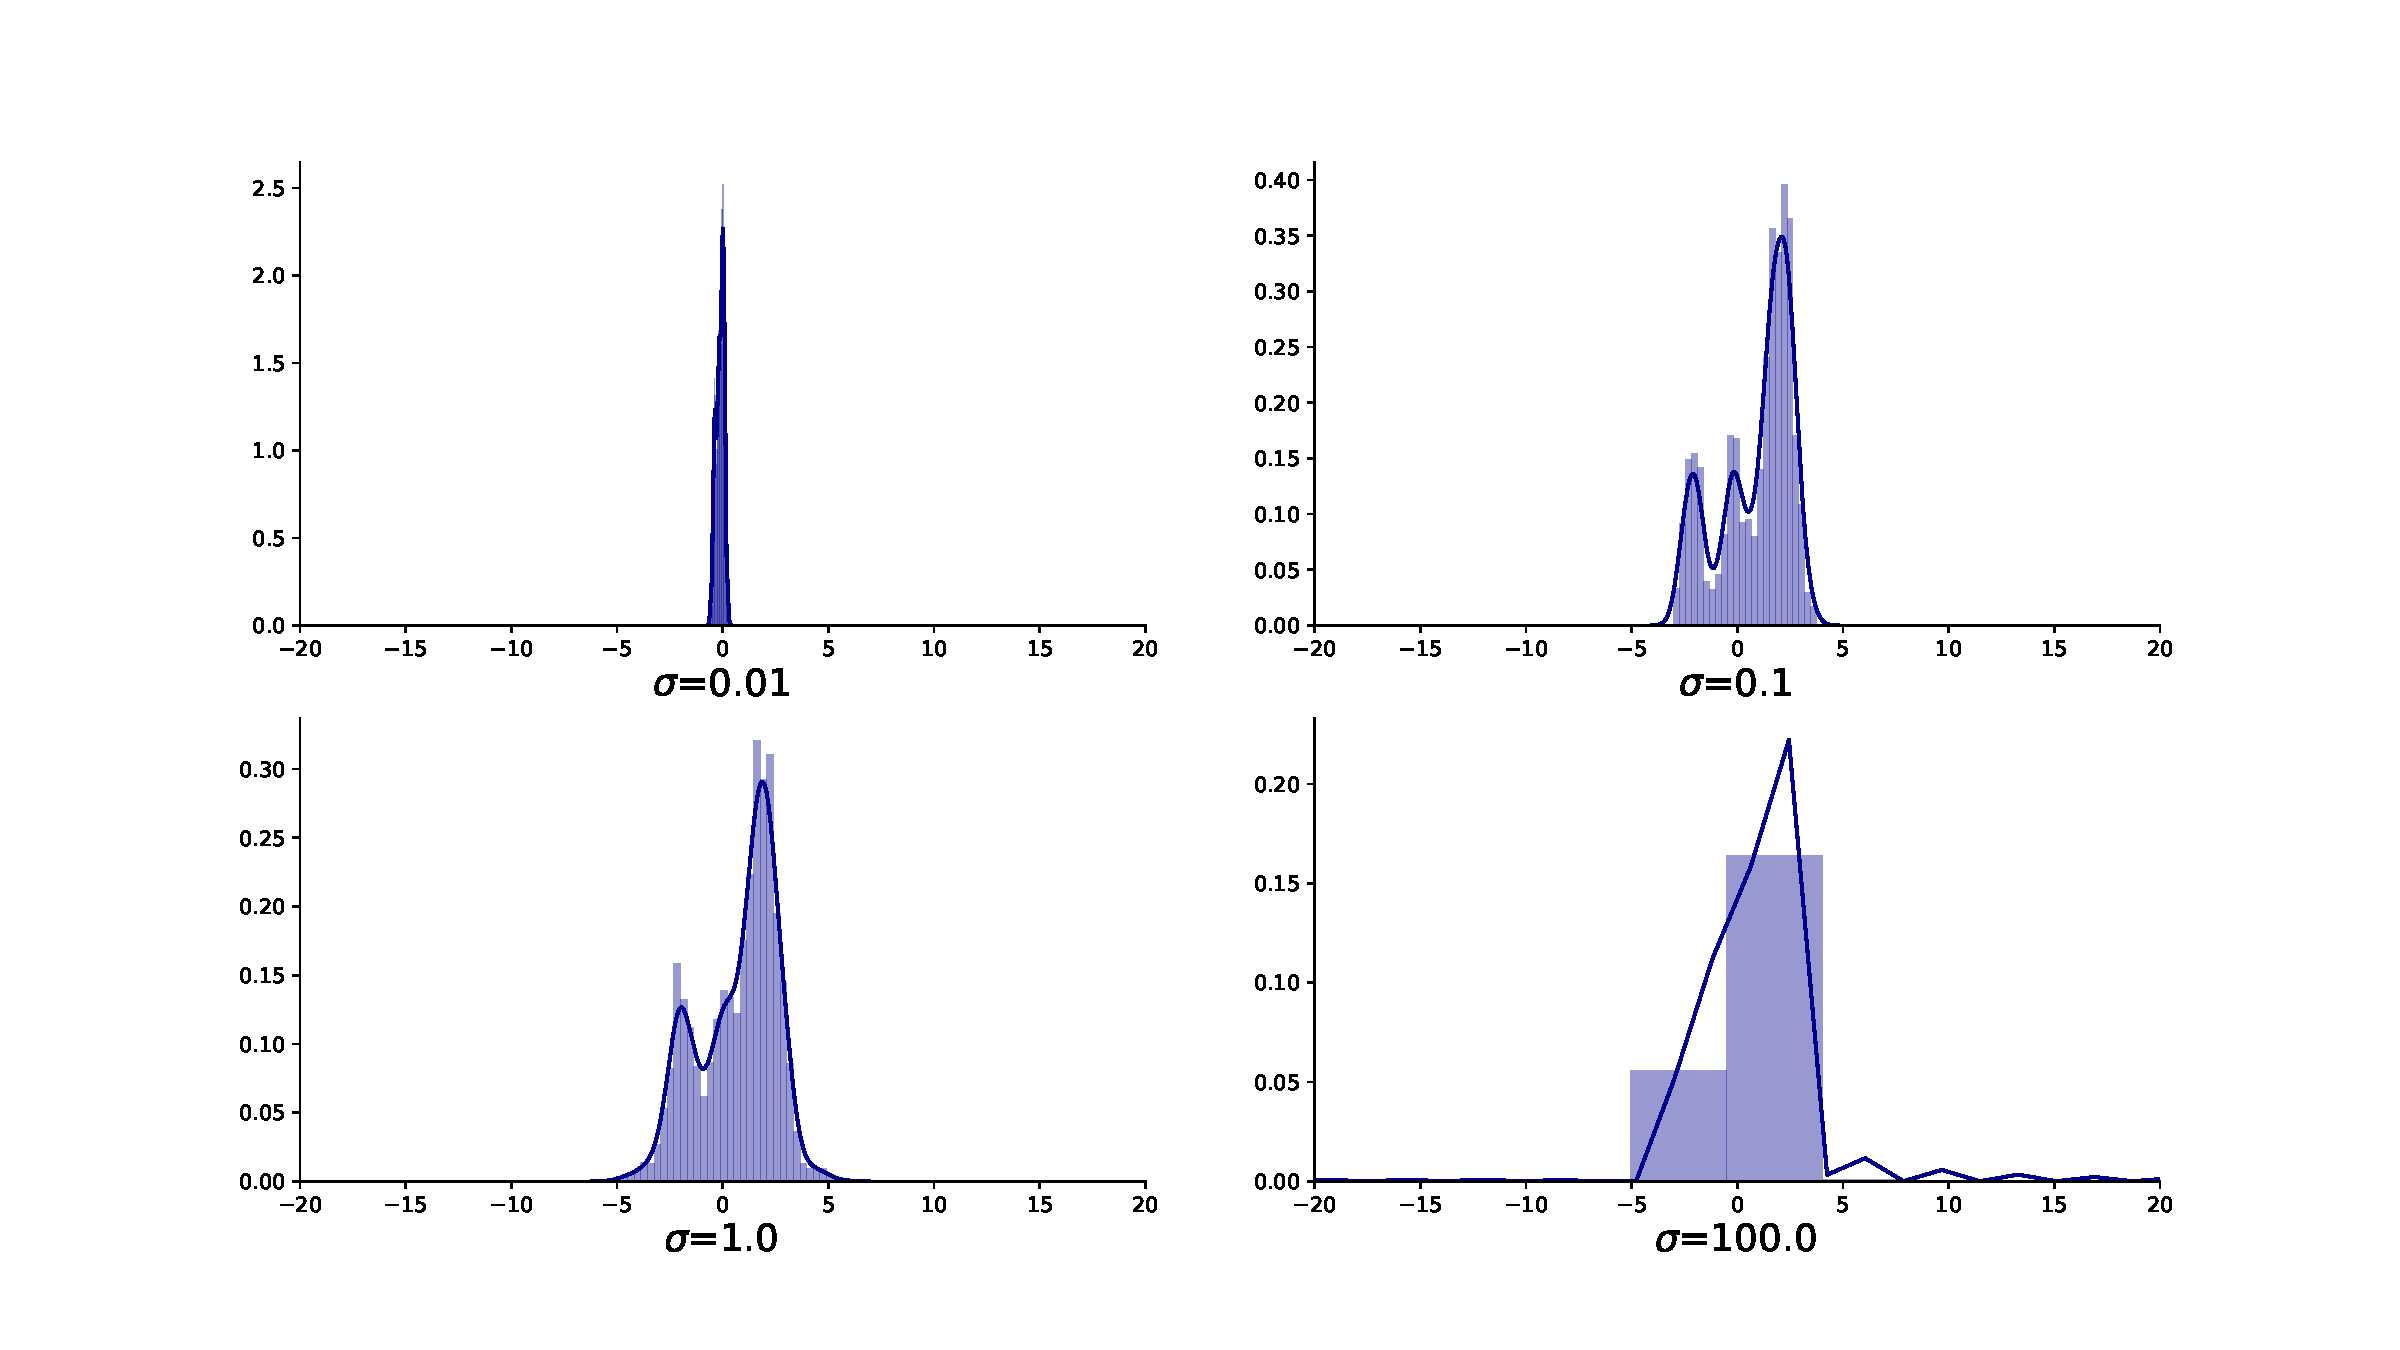
\includegraphics[width=0.5\textwidth]{img/metrepolis_hastings.pdf} 
    \caption{Approximations obtained using the MH algorithm with Gaussian proposal with different stanrdar deviation $\sigma$.}
\end{figure}

The output of the MH algotithm can be used for point estimation, estimating quantities as mean, median or mode (the point with highest density). However, that method is not much efficient to estimate the mode because the random samples solely rarely come from the vicinity of the mode. A better way to do that is Simulated Annealing (SA). This method sampling from $p^{1/T_{i}}(x)$ instead of $p(x)$. The term $T_{i}$ is a decreasing cooling schedule with $\lim_{i\rightarrow \infty} T_{i} = 0$. To estimate the mode of $p(x)$ we set $T_{i} = Cln(i+T_{0})$, with $T_{0}=1$ and $C=2$, in this manner the series is decreasing. The result of applying SA to the previous example are shown in Figure 2. In this case the better approximation apparently is reached by $\sigma=1$, where the mode is 1.95. In brief, to obtain efficient annealed algorithms, it is again important to choose suitable proposal distributions and an appropiate cooling schedule.

\begin{figure}[!h]
    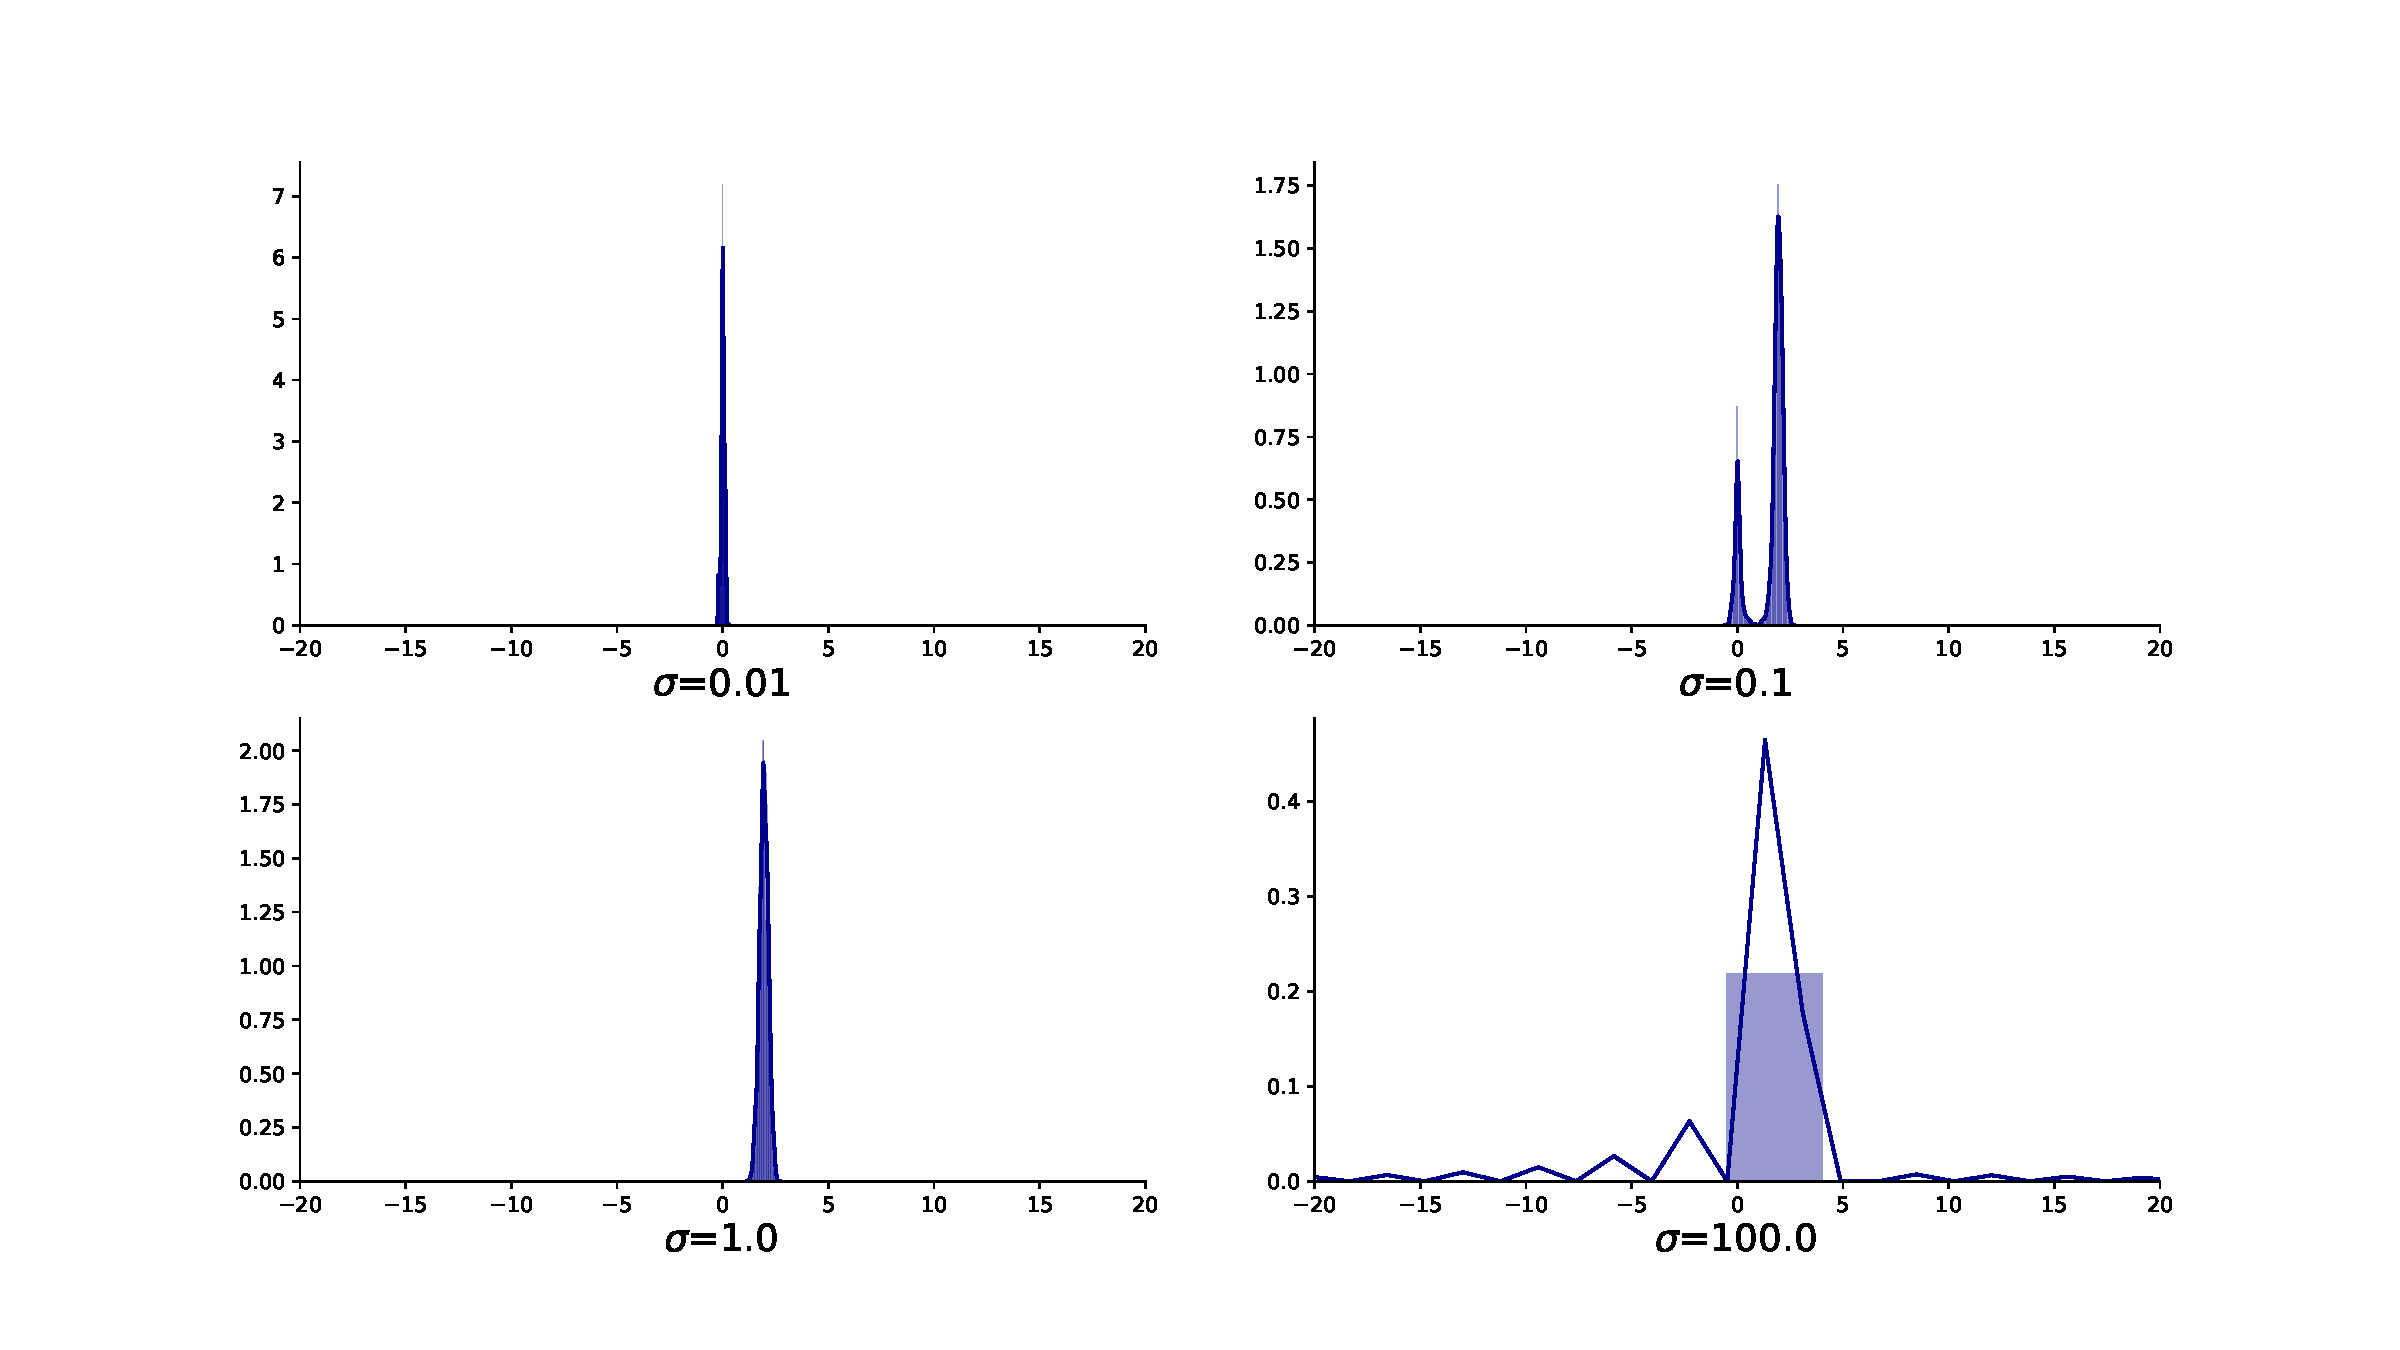
\includegraphics[width=0.5\textwidth]{img/simulated_annealing.pdf} 
    \caption{Discovering the modes of the target distribution using the SA algorithm.}
\end{figure}

\section{Gibbs Sampling}

In this section we use the Gibbs Sampling (GB) algorithm to empirically approximate $p(z,\pi, \mu|x)$, where $x=x_{1}, \ldots, x_{100}$ is the data, $z=z_{1}, \ldots, z_{100}$ are the hiddens variables, in this case are the binary cluster assignments, $\pi$ is the mixture proportion, and $\mu=[\mu_{0}, \mu_{1}]$ are the parameters of the observation model. The generative process is detailed below: 

\begin{align}
\mu_{0}, \mu_{1} &\sim \mathcal{N}(0,5)\\
\pi&\sim Beta(0.8,0.8)\\
z_{1}, \ldots, z_{100}|\mu, \pi &\sim Bernoulli(\pi)\\
z_{i} &\sim \mathcal{N}(\mu_{z_{i}, 0.25}) 
\end{align}

Firstly, we generate a random sample from this process. In this case the resulting main parameters are $\mu_{0}=2.357$, $mu_{1}=-5.955$ and $\pi=0.788$. This is ilustrated in Figure 3. Secondly, is necessary to get the full conditional distribution $p(z_{i}|z_{-i}, \pi, \mu, x)$, $p(\mu_{k}|z, \pi, \mu_{-k}, x)$ and $p(\pi|z, \mu, x)$. The variable $z_{i}$ is conditional independent from $z_{-i}$ and $x_{-i}$ given $x_{i}$, so $p(z_{i}|z_{-i}, \pi, \mu, x)$ can be written as follows

\begin{align}
p(z_{i}=0|\pi, \mu, x_{i}) &=  (1-\pi) \mathcal{N}(x_{i}|\mu_{0}, 0.25) = \alpha_{0}\\
p(z_{i}=1|\pi, \mu, x_{i}) &=  \pi \mathcal{N}(x_{i}|\mu_{1}, 0.25) = \alpha_{1}\\
p(z_{i}|\pi, \mu, x_{i}) &\sim Bernoulli(\frac{\alpha_{1}}{\alpha_{0}+\alpha_{1}})
\end{align}

; the variable $\pi$ is conditional independent from $\mu$ and $x$ given $z$, then the full conditional is

\begin{align}
    p(\pi|z, \mu, x) &= Beta(0.8+N_{1}, 0.8+N_{0})\\
    N_{0} = \sum_{i=1, z_{i}=0}^{100}1&, \; N_{1} = \sum_{i=1, z_{i}=1}^{100}1
\end{align}

; and $\mu_{i}$ is independent from $\mu_{-i}$ and $\pi$ given $z$ and $x$, then the full conditional is
\begin{align}
    \sigma_{0}^{2} = \bigg(\frac{1}{5^{2}}+\frac{N_{0}}{0.25^{2}}\bigg)^{-1}&, \; \sigma_{1}^{2} = \bigg(\frac{1}{5^{2}}+\frac{N_{1}}{0.25^{2}}\bigg)^{-1}\\
    m_{0} = \sigma_{0}^{2}\bigg(\frac{\sum_{i=1, z_{i}=0}^{100}x_{i}}{0.25^{2}}\bigg)&, \; m_{1} = \sigma_{1}^{2}\bigg(\frac{\sum_{i=1, z_{i}=1}^{100}x_{i}}{0.25^{2}}\bigg)\\
    p(\mu_{0}|z, x) \sim \mathcal{N}(m_{0}, \sigma_{0}) &, \; p(\mu_{1}|z, x) \sim \mathcal{N}(m_{1}, \sigma_{1})
\end{align}
With all previous full conditionals we can implement the Gibbs sampling algorithm.


Finally, the results  is illustrated in Figure 4-5, where we can observe that the algorithms fastly converge to a negihborhood of the target parameters used to draw the data. The expected value approximation, i.e., the sample mean, are $\pi=0.770$, $\mu_{0}=2.275$ and $\mu_{1}=-5.954$, very close to the original values. To sum up, the Gibbs Sampling algorithm is an excellent algorithm to approximate complicated densities with a directed graph structure that encodes the conditional indepedencies in the model.


\begin{figure}[!h]
    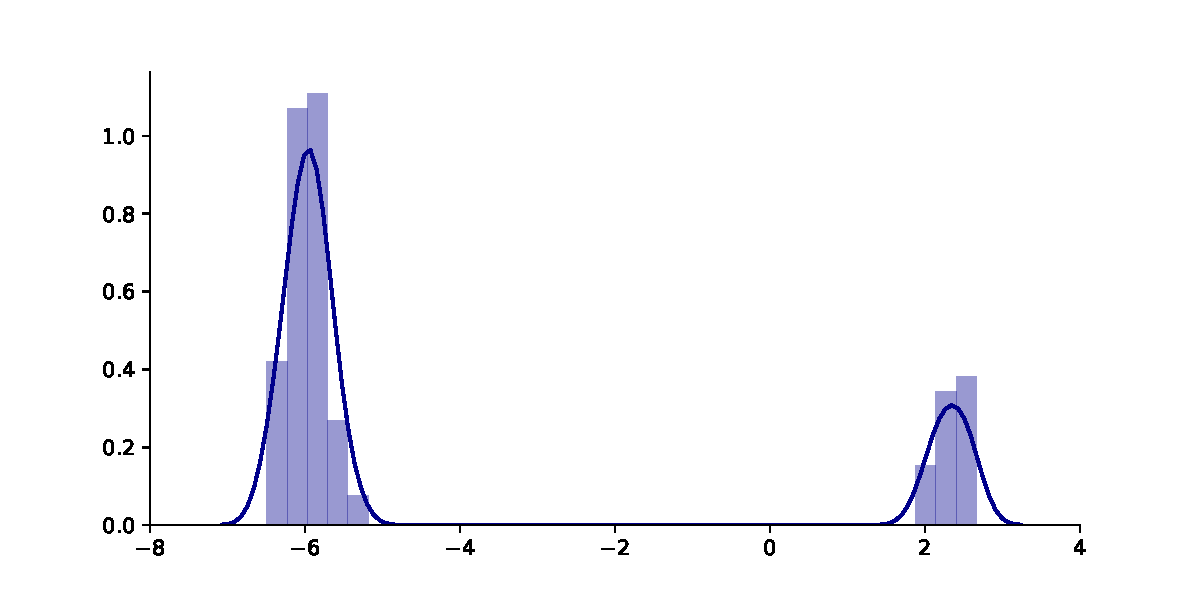
\includegraphics[width=0.5\textwidth]{img/gaussian_mixture.pdf} 
    \caption{Random sample of a mixture of two Gaussians.}
\end{figure}

\begin{figure}[!h]
    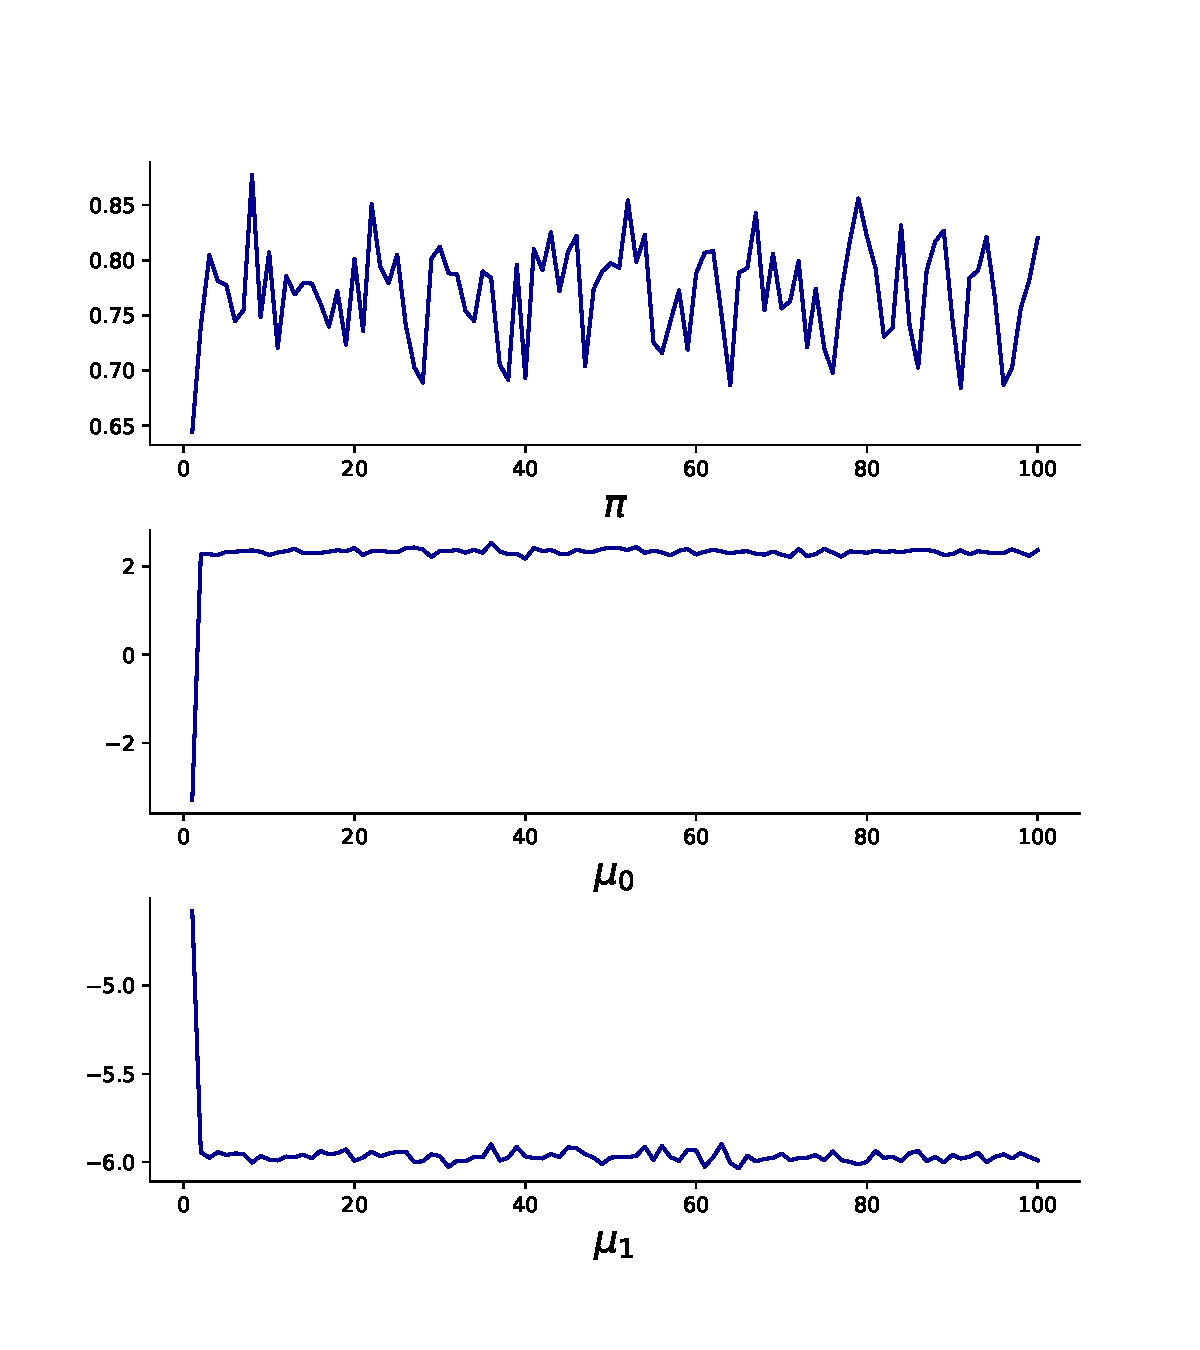
\includegraphics[width=0.5\textwidth]{img/gibbs_sampling_walk.pdf} 
    \caption{Posterior samples drawn from the Gibbs Sampling algorithm.}
\end{figure}

\begin{figure}[!h]
    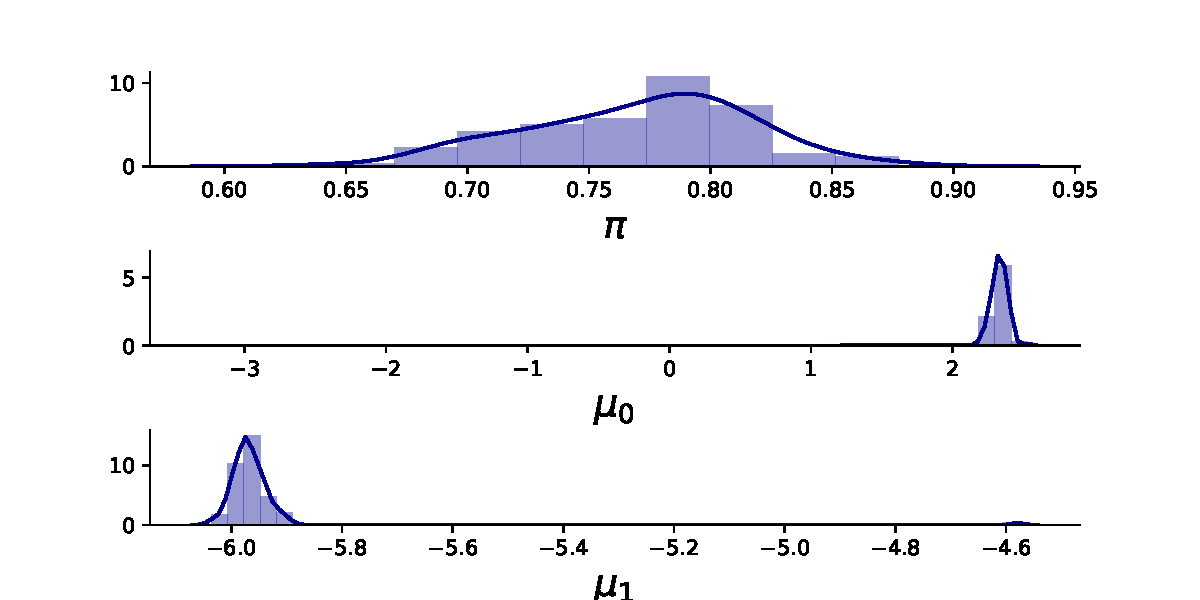
\includegraphics[width=0.5\textwidth]{img/gibbs_sampling_density.pdf} 
    \caption{Posterior approximation from the Gibbs Sampling algorithm.}
\end{figure}

\end{document}